\documentclass{standalone}
\usepackage{tikz}
\usetikzlibrary{patterns, positioning}

\begin{document}
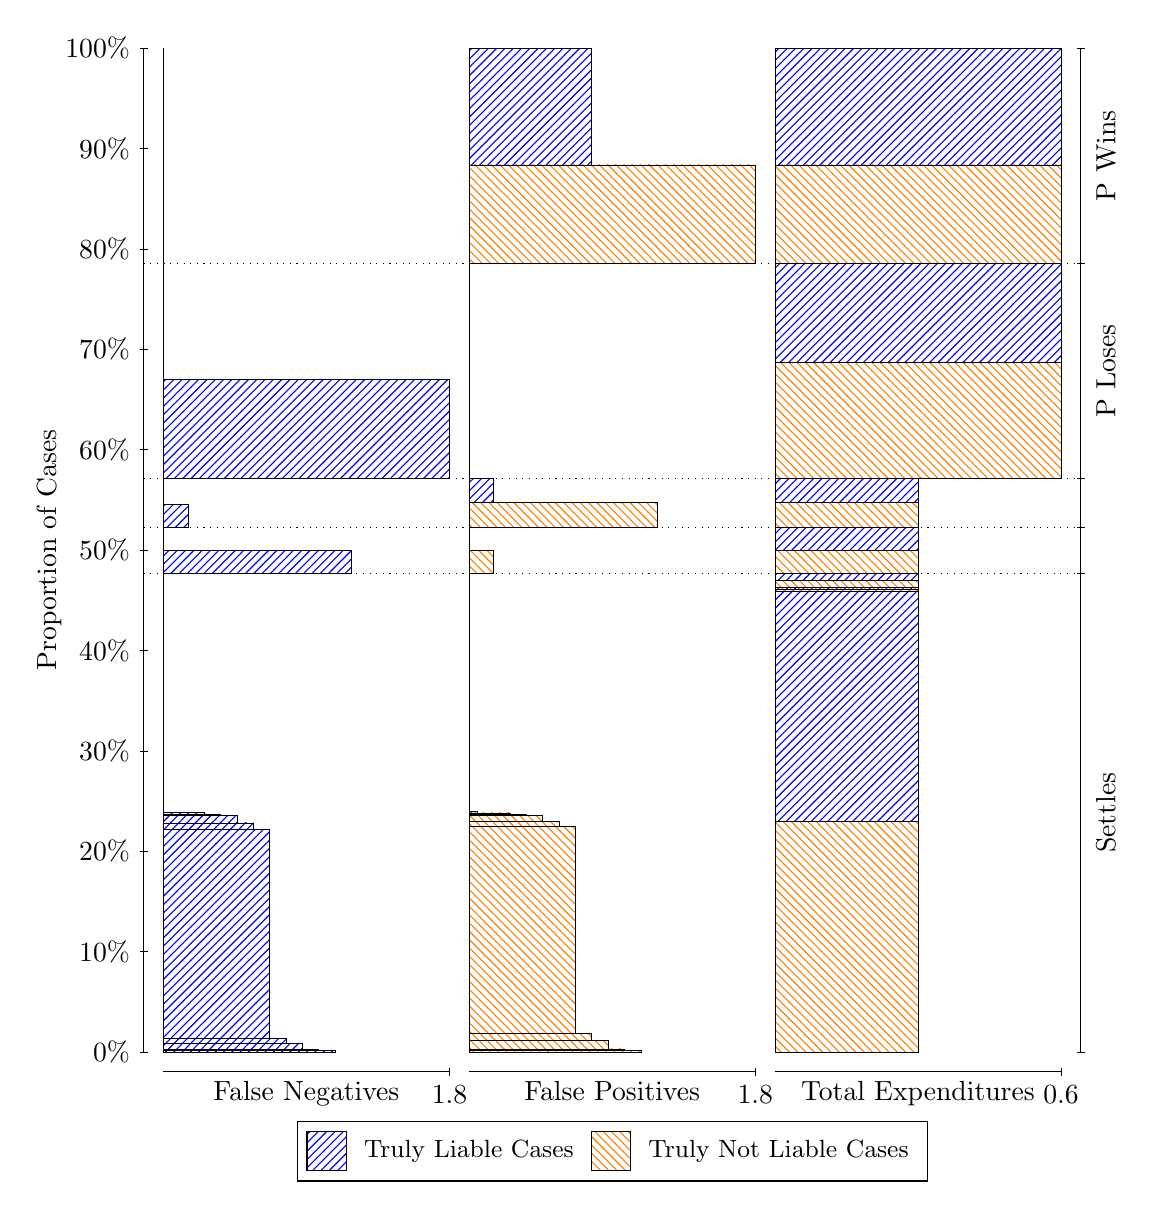
\begin{tikzpicture}
\draw[black, very thin] (1.5,1.75) -- (1.5,14.5);
\node[rotate=90, anchor=center] at (0.3, 8.125) {Proportion of Cases};
\draw[black, very thin] (1.45,1.75) -- (1.55,1.75);
\node[anchor=east] at (1.45, 1.75) {0\%};
\draw[black, very thin] (1.45,3.025) -- (1.55,3.025);
\node[anchor=east] at (1.45, 3.025) {10\%};
\draw[black, very thin] (1.45,4.3) -- (1.55,4.3);
\node[anchor=east] at (1.45, 4.3) {20\%};
\draw[black, very thin] (1.45,5.575) -- (1.55,5.575);
\node[anchor=east] at (1.45, 5.575) {30\%};
\draw[black, very thin] (1.45,6.85) -- (1.55,6.85);
\node[anchor=east] at (1.45, 6.85) {40\%};
\draw[black, very thin] (1.45,8.125) -- (1.55,8.125);
\node[anchor=east] at (1.45, 8.125) {50\%};
\draw[black, very thin] (1.45,9.4) -- (1.55,9.4);
\node[anchor=east] at (1.45, 9.4) {60\%};
\draw[black, very thin] (1.45,10.675) -- (1.55,10.675);
\node[anchor=east] at (1.45, 10.675) {70\%};
\draw[black, very thin] (1.45,11.95) -- (1.55,11.95);
\node[anchor=east] at (1.45, 11.95) {80\%};
\draw[black, very thin] (1.45,13.225) -- (1.55,13.225);
\node[anchor=east] at (1.45, 13.225) {90\%};
\draw[black, very thin] (1.45,14.5) -- (1.55,14.5);
\node[anchor=east] at (1.45, 14.5) {100\%};

\draw[black, very thin] (13.4,1.75) -- (13.4,14.5);
\draw[black, very thin] (13.35,1.75) -- (13.45,1.75);
\node[anchor=west] at (13.35, 1.75) {};
\draw[black, very thin] (13.35,7.8284) -- (13.45,7.8284);
\node[anchor=west] at (13.35, 7.8284) {};
\draw[black, very thin] (13.35,8.4077) -- (13.45,8.4077);
\node[anchor=west] at (13.35, 8.4077) {};
\draw[black, very thin] (13.35,9.0303) -- (13.45,9.0303);
\node[anchor=west] at (13.35, 9.0303) {};
\draw[black, very thin] (13.35,11.764) -- (13.45,11.764);
\node[anchor=west] at (13.35, 11.764) {};
\draw[black, very thin] (13.35,14.5) -- (13.45,14.5);
\node[anchor=west] at (13.35, 14.5) {};

\draw[black, very thin, pattern color=blue, pattern=north east lines] (1.75,1.75) rectangle (3.93,1.7737);
\draw[black, very thin, pattern color=blue, pattern=north east lines] (1.75,1.7737) rectangle (3.7224,1.7845);
\draw[black, very thin, pattern color=blue, pattern=north east lines] (1.75,1.7845) rectangle (3.5148,1.8595);
\draw[black, very thin, pattern color=blue, pattern=north east lines] (1.75,1.8595) rectangle (3.3071,1.9255);
\draw[black, very thin, pattern color=blue, pattern=north east lines] (1.75,1.9255) rectangle (3.0995,4.5782);
\draw[black, very thin, pattern color=blue, pattern=north east lines] (1.75,4.5782) rectangle (2.8919,4.6592);
\draw[black, very thin, pattern color=blue, pattern=north east lines] (1.75,4.6592) rectangle (2.6843,4.755);
\draw[black, very thin, pattern color=blue, pattern=north east lines] (1.75,4.755) rectangle (2.4767,4.7722);
\draw[black, very thin, pattern color=blue, pattern=north east lines] (1.75,4.7722) rectangle (2.269,4.7911);
\draw[black, very thin, pattern color=orange, pattern=north west lines] (1.75,4.7911) rectangle (1.75,7.8284);
\draw[black, very thin, pattern color=blue, pattern=north east lines] (1.75,7.8284) rectangle (4.1376,8.1194);
\draw[black, very thin, pattern color=orange, pattern=north west lines] (1.75,8.1194) rectangle (1.75,8.4077);
\draw[black, very thin, pattern color=blue, pattern=north east lines] (1.75,8.4077) rectangle (2.0614,8.7055);
\draw[black, very thin, pattern color=orange, pattern=north west lines] (1.75,8.7055) rectangle (1.75,9.0303);
\draw[black, very thin, pattern color=blue, pattern=north east lines] (1.75,9.0303) rectangle (5.3833,10.291);
\draw[black, very thin, pattern color=orange, pattern=north west lines] (1.75,10.291) rectangle (1.75,11.764);
\draw[black, very thin, pattern color=orange, pattern=north west lines] (1.75,11.764) rectangle (1.75,13.015);
\draw[black, very thin, pattern color=blue, pattern=north east lines] (1.75,13.015) rectangle (1.75,14.5);
\draw[black, very thin, pattern color=orange, pattern=north west lines] (5.6333,1.75) rectangle (7.8133,1.7699);
\draw[black, very thin, pattern color=orange, pattern=north west lines] (5.6333,1.7699) rectangle (7.6057,1.7891);
\draw[black, very thin, pattern color=orange, pattern=north west lines] (5.6333,1.7891) rectangle (7.3981,1.8938);
\draw[black, very thin, pattern color=orange, pattern=north west lines] (5.6333,1.8938) rectangle (7.1905,1.9819);
\draw[black, very thin, pattern color=orange, pattern=north west lines] (5.6333,1.9819) rectangle (6.9829,4.6142);
\draw[black, very thin, pattern color=orange, pattern=north west lines] (5.6333,4.6142) rectangle (6.7752,4.6772);
\draw[black, very thin, pattern color=orange, pattern=north west lines] (5.6333,4.6772) rectangle (6.7752,4.6793);
\draw[black, very thin, pattern color=orange, pattern=north west lines] (5.6333,4.6793) rectangle (6.5676,4.7529);
\draw[black, very thin, pattern color=orange, pattern=north west lines] (5.6333,4.7529) rectangle (6.36,4.7634);
\draw[black, very thin, pattern color=orange, pattern=north west lines] (5.6333,4.7634) rectangle (6.1524,4.7873);
\draw[black, very thin, pattern color=blue, pattern=north east lines] (5.6333,4.7873) rectangle (5.7371,4.8062);
\draw[black, very thin, pattern color=blue, pattern=north east lines] (5.6333,4.8062) rectangle (5.6333,7.8284);
\draw[black, very thin, pattern color=orange, pattern=north west lines] (5.6333,7.8284) rectangle (5.9448,8.1166);
\draw[black, very thin, pattern color=blue, pattern=north east lines] (5.6333,8.1166) rectangle (5.6333,8.4077);
\draw[black, very thin, pattern color=orange, pattern=north west lines] (5.6333,8.4077) rectangle (8.021,8.7325);
\draw[black, very thin, pattern color=blue, pattern=north east lines] (5.6333,8.7325) rectangle (5.9448,9.0303);
\draw[black, very thin, pattern color=orange, pattern=north west lines] (5.6333,9.0303) rectangle (5.6333,10.503);
\draw[black, very thin, pattern color=blue, pattern=north east lines] (5.6333,10.503) rectangle (5.6333,11.764);
\draw[black, very thin, pattern color=orange, pattern=north west lines] (5.6333,11.764) rectangle (9.2667,13.015);
\draw[black, very thin, pattern color=blue, pattern=north east lines] (5.6333,13.015) rectangle (7.1905,14.5);
\draw[black, very thin, pattern color=orange, pattern=north west lines] (9.5167,1.75) rectangle (11.333,4.6772);
\draw[black, very thin, pattern color=blue, pattern=north east lines] (9.5167,4.6772) rectangle (11.333,7.6069);
\draw[black, very thin, pattern color=orange, pattern=north west lines] (9.5167,7.6069) rectangle (11.333,7.6308);
\draw[black, very thin, pattern color=blue, pattern=north east lines] (9.5167,7.6308) rectangle (11.333,7.6545);
\draw[black, very thin, pattern color=orange, pattern=north west lines] (9.5167,7.6545) rectangle (11.333,7.7407);
\draw[black, very thin, pattern color=blue, pattern=north east lines] (9.5167,7.7407) rectangle (11.333,7.8284);
\draw[black, very thin, pattern color=orange, pattern=north west lines] (9.5167,7.8284) rectangle (11.333,8.1166);
\draw[black, very thin, pattern color=blue, pattern=north east lines] (9.5167,8.1166) rectangle (11.333,8.4077);
\draw[black, very thin, pattern color=orange, pattern=north west lines] (9.5167,8.4077) rectangle (11.333,8.7325);
\draw[black, very thin, pattern color=blue, pattern=north east lines] (9.5167,8.7325) rectangle (11.333,9.0303);
\draw[black, very thin, pattern color=orange, pattern=north west lines] (9.5167,9.0303) rectangle (13.15,10.503);
\draw[black, very thin, pattern color=blue, pattern=north east lines] (9.5167,10.503) rectangle (13.15,11.764);
\draw[black, very thin, pattern color=orange, pattern=north west lines] (9.5167,11.764) rectangle (13.15,13.015);
\draw[black, very thin, pattern color=blue, pattern=north east lines] (9.5167,13.015) rectangle (13.15,14.5);
\draw[black, dotted] (1.5,7.8284) -- (13.4,7.8284);
\draw[black, dotted] (1.5,8.4077) -- (13.4,8.4077);
\draw[black, dotted] (1.5,9.0303) -- (13.4,9.0303);
\draw[black, dotted] (1.5,11.764) -- (13.4,11.764);
\draw[black, very thin] (1.75,1.5) -- (5.3833,1.5);
\node[anchor=north] at (3.5667, 1.5) {False Negatives};
\draw[black, very thin] (5.3833,1.45) -- (5.3833,1.55);
\node[anchor=north] at (5.3833, 1.45) {1.8};

\draw[black, very thin] (5.6333,1.5) -- (9.2667,1.5);
\node[anchor=north] at (7.45, 1.5) {False Positives};
\draw[black, very thin] (9.2667,1.45) -- (9.2667,1.55);
\node[anchor=north] at (9.2667, 1.45) {1.8};

\draw[black, very thin] (9.5167,1.5) -- (13.15,1.5);
\node[anchor=north] at (11.333, 1.5) {Total Expenditures};
\draw[black, very thin] (13.15,1.45) -- (13.15,1.55);
\node[anchor=north] at (13.15, 1.45) {0.6};

\node[black, centered, rotate=90] at (13.72, 4.7892) {Settles};


\node[black, centered, rotate=90] at (13.72, 10.397) {P Loses};
\node[black, centered, rotate=90] at (13.72, 13.132) {P Wins};

\draw (7.449999999999999,1.5) node[draw=none] (baseCoordinate) {};
\begin{scope}[align=center]
        \matrix[scale=0.5, draw=black, below=0.5cm of baseCoordinate, nodes={draw}, column sep=0.1cm]{
            \node[rectangle, draw, minimum width=0.5cm, minimum height=0.5cm, pattern=north east lines, pattern color=blue] {}; &
            \node[draw=none, font=\small] (B) {Truly Liable Cases}; &
            \node[rectangle, draw, minimum width=0.5cm, minimum height=0.5cm, pattern=north west lines, pattern color=orange] {}; &
            \node[draw=none, font=\small] (B) {Truly Not Liable Cases}; \\
            };
\end{scope}

\end{tikzpicture}
\end{document}